%!TEX root = ../PhDthesis.tex
\chapter{Long-range interactions in the visual cortex}

One of the most striking features in the early visual cortex is the
presence of patchy long-range excitatory connections linking regions
with similar feature preferences. These connections have been
suggested to drive a wide range of contextual modulation effects
including pop-out, iso-orientation suppression, contour completion and
more \citep{Gilbert1983, Hirsch1991, McGuire1991, Grinvald1994,
  Fitzpatrick2000, Hupe2001, Stettler2002}. Even though these
connections are excitatory it is now well established that they also
provide inhibition via a di- or poly-synaptic mechanism
\citep{Weliky1995}. While both the SCAL and SEPI models optionally
have long-range excitation these connections, since these connections
are purely excitatory they cannot mediate long-range suppressive
effects directly and due to the weakly tuned nature of the PV cell
population they too are not viable candidates to mediate feature
specific contextual modulation effects such as iso-orientation
suppression.

A major feature of the neural code in the cortex is the elimination of
redundancy in order to achieve a sparse representation of the input
\citep{Olshausen1996}. Indeed it has been found that modulation from
the nonclassical receptive field suppresses redundant information in
the input sparsifying the neural code \citep{Vinje2000}. In previous
developmental models of the primary visual cortex it was shown that
allowing lateral inhibitory connections to develop non-isotropic
connectivity, which allows the network to learn the redundant features
of the input and suppress them, results in a sparser representation
\citep{Miikkulainen2005b}. If such development is not allowed to take
place and isotropic surround suppression is employed,
cross-orientation stimuli, belonging to a separate object or contour
may be suppressed, thus reducing the information content encoded by
the network.

This suggests a difference between short scale interactions where the
cortex is trying to ensure it achieves maximal coverage of the feature
space and long-range interactions where the neuron is competing to
represent the stimulus itself in an efficient way, i.e. by using a
sparse code. In the previous models the PV inhibition drove the local
competition resulting in a smooth coverage of the visual space with
orientation feature detectors, i.e. an orientation map. Since these
neurons act over a fairly small range and are not highly tuned in the
orientation domain they are generally isotropic in the spatial
distribution and cannot mediate feature specific modulation.

In the literature we have identified a second population of inhibitory
interneurons with interesting properties. The Somatostatin
immunoreactive (Sst) neurons are the second largest group of
interneurons \citep{Gonchar2007,Xu2010} and exhibit very different
properties from the PV population, which makes them interesting as a
candidate to perform long-range integration of inputs. Specifically
they are enriched in layer 2/3 where a lot of the long-range patchy
connectivity is found and they seem to respond strongly only under
strong, sustained stimulation \citep{Ma2011} or for very large stimuli
\citep{Adesnik2012}. Additionally the input scaling does not seem to
be linear, with a accelerating response function driving much stronger
responses when they recruited consistently and robustly (as would be
the case for large or high contrast stimuli)
\citep{Beierlein2003,Bartley2008,Tan2008}.

On the basis of what we have learned about the PV population from the
previous models and what we know about Somatostatin neurons from the
literature we therefore propose a general theory of how the circuit
performs specific computations. Afferent input provides strong,
low-latency excitation to the Pv-ir neurons in the thalamocortical
recipient layer 4, which in turn act as both a feedforward inhibition
and dynamic gain control mechanism on the broadly activated excitatory
cell population. This results in local decorrelation of the neural
activity, which allows recurrent excitation to amplify the activity in
the local neural ensemble, which leads to the formation of a smooth
orientation map.

At the same time Sst-ir neurons begin to integrate the local activity
through the local and long-range orientation-specific lateral
connections. If their inputs are sufficiently strong they will
activate strongly allowing this polysynaptic circuit to reduce
long-range correlation in the input activity, further reducing
redundancy. If they are only weakly activated, as would occur when
presented with low-contrast or very sparse input patterns, long-range
lateral excitatory connections are not outcompeted and the circuit can
fill in weak or missing information based on past statistics. In such
a regime the differential recruitment of the two separate inhibitory
populations would be responsible for a shift in cortical state from a
mode of redundancy-reduction and feature discrimination to one of
visual inference.

In this chapter we further extend the existing SEPI model by adding
this second population of inhibitory neurons modelled after the Sst
interneuron population. In doing so we will demonstrate how this
second population integrates large and high-contrast stimuli providing
feature specific inhibition under those conditions, while only very
weakly responding in low contrast conditions. This provides a
considerable advance over previous models, which differ in that they
usually hard-code the statistical relationships encoded in the lateral
connections and generally explain contrast dependent changes through a
higher inhibitory threshold, which is generally not supported by
evidence. The contextual modulation effects are therefore an emergent
phenomenon, arising from the correlations present in the training
patterns. Identifying and modeling the circuits involved in these
processes is a fundamental challenge for neuroscience and will hugely
contribute to extending our understanding of cortical information
processing.

\section{Methods}

\subsection{The LESPI model}

The \textbf{L}ong-\textbf{R}ange \textbf{E}xcitation, \textbf{S}sst
and \textbf{PV} \textbf{I}nhibition (LESPI) model again builds on the
previous models introducing an additional population of inhibitory
neurons, which is entirely recurrently driven via short- and
long-range projections by the two other populations. The diagram in
\ref{LESPIDiagram} shows how the three populations of V1 neurons are
recurrently connected.

The newly introduced Sst population will differ from the PV population
in a number of respects. First of all it receives no afferent input
from the LGN, as this population is thought to be enriched in
supra-granular layers, which do not receive direct afferent
input. Secondly this population has a much more restricted spatial
profile being not nearly as extensive in their lateral extent as the
PV expressing basket cells. Most importantly however the facilitating
response properties of lateral synaptic connections contacting this
population is modeled via an exponential non-linearity in their
response. This allows this population to activate weakly in
low-contrast conditions, while providing strong suppression when the
input is strong or dense enough. Finally to model the more sluggish
responses among this population a hysteresis term is added. In this
way this population responds strongly after sustained and strong local
and long-range stimulation.

\subsubsection{Excitatory Activation}

The influence of the aggregate long-range excitatory and di-synaptic
inhibition via the Sst population is expressed as an additional
multiplicative factor modulating the response of the excitatory
neurons. The response of the excitatory population is then given by:

\begin{equation}
  \eta_{exc} = \frac{\eta_{A} + \eta_{LOC-EXC}}{1 + \eta_{PV-INH}} \eta_{SM}
\end{equation}

where $\eta_{A}$ is the LGN afferent activity, $\eta_{LOC-EXC}$ the local
excitatory contribution, $\eta_{PV-INH}$ the PV inhibitory contribution
and the surround-modulation term $\eta_{SM}$ is defined as:

\begin{equation}
  \eta_{SM} = 1 + \eta_{LAT-EXC} - \eta_{Sst}
\end{equation}

where $\eta_{LAT-EXC}$ represents the long-range lateral excitatory
contribution and $\eta_{Sst}$ is the Sst inhibitory contribution. In
the SEPI model the $\eta_{SM}$ term simply reduces to 1, eliminating
all long-range interactions. The surround-modulation term provides
gain when excitation exceeds inhibition and shunting inhibition when
the reverse is true. As such, this term provides a convenient
abstraction to model the modulatory influence of the dendritic
integration of long-range inputs, although in reality they will
provide both multiplicative/divisive and additive/subtractive effects.

\subsubsection{Inhibitory Sst Activation}

The activation of the inhibitory Sst population is given simply by the
summation of the local and lateral excitatory projection activity:

\begin{equation}
  \eta_{Sst} = \eta_{LOC-EXC} + \eta_{LAT-EXC}
\end{equation}

Additionally the $\eta_{LAT-EXC}$ term has an exponential activation
function applied to it such that it's contribution is given by

\subsubsection{Mechanisms}

The effective excitatory gain may not be a bad approximation to the
effect of long-range horizontal connections, which have been shown to
be strongly voltage dependent \citep{Hirsch1991}. Since Sst neurons
generally target distal dendrites they have generally been associated
with subtractive inhibition, they do however also have a
multiplicative component \citep{Wilson2012}. Additionally, their
preference for targetting distal dendrites may allow them to
effectively gate horizontal excitatory and feedback inputs
\citep{Ma2011, Gentet2012}. Additionally theoretical studies indicate
active dendritic spike backpropagation can lead to multiplicative
increases in gain, while reduction in spike backpropagation can lead
to divisive scaling of the firing rate \citep{Mehaffey2005}.

\begin{figure}
	\centering
        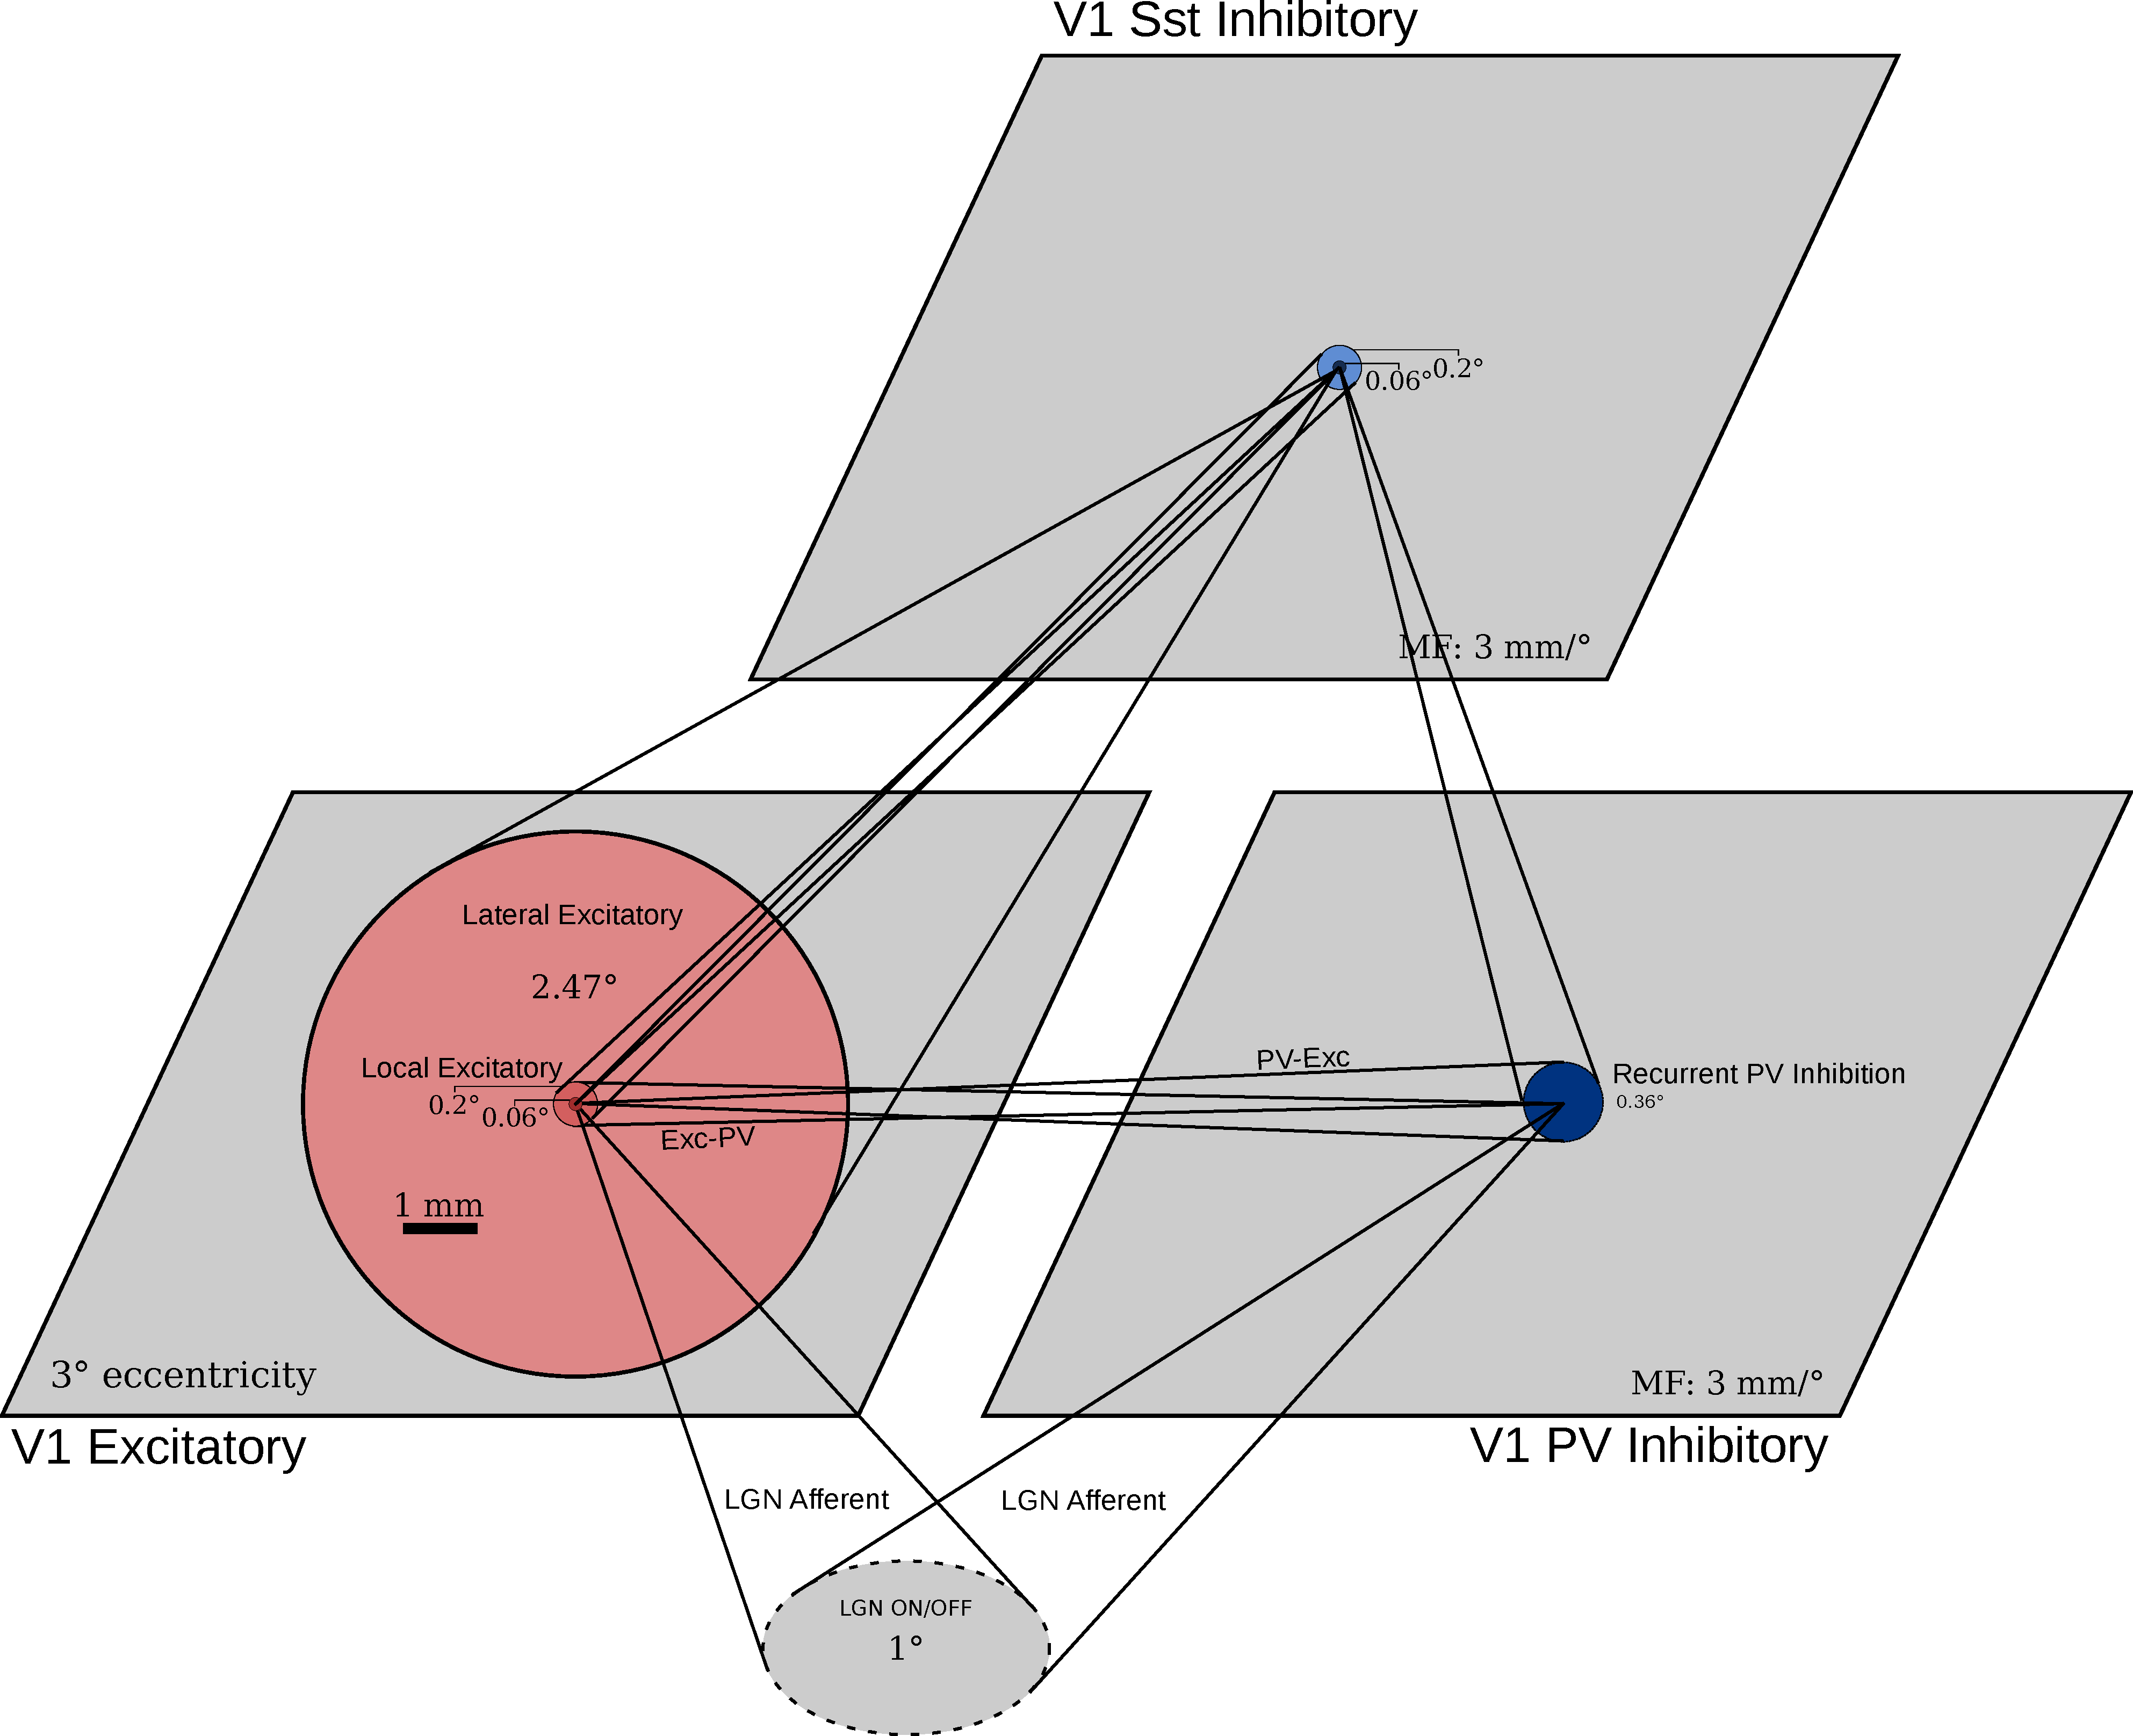
\includegraphics[width=1.0\textwidth]{LESPI_Diagram.pdf}
	\caption{Diagram of the LESPI V1 stage of the model showing the
          spatial scales of the various excitatory (red) and
          inhibitory (blue) connections. Satured colors indicate the
          kernel radii, while lightly shaded regions indicate kernel
          cut-off extents.}
	\label{LESPIDiagram}
\end{figure}

The overall operation of this circuit can be summarized by the
schematic in \ref{circuit_diagram}. The diagram shows the preferential
linking of columns with similar orientation preference via patchy
long-range connections and the long-range integration of Sst neurons,
which receive both local and lateral input from pyramidal neurons,
providing di-synaptic inhibition to the local region. Furthermore it
suggests that under low-contrast conditions the Sst population is
effectively disabled, activating only under high contrast input.

\begin{figure}
	\centering
	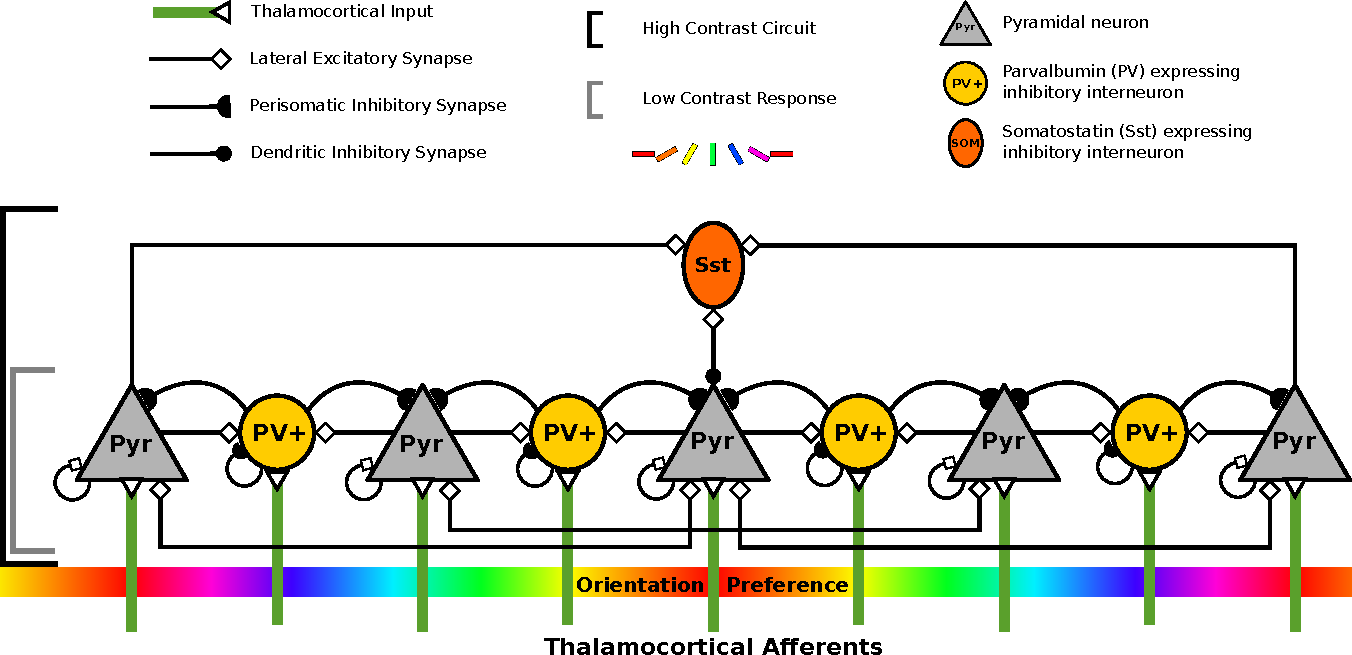
\includegraphics[width=1.0\textwidth]{./v1circuit.pdf}
	\caption[High-level circuit diagram of the LESPI
      model.]{High-level circuit diagram of the LESPI model. The
      schematic represents multiple hypercolumns varying smoothly in
      their orientation preference. PV neurons provide feedforward and
      recurrent inhibition to neurons to columns in the local region,
      regardless of their orientation tuning. Long-range excitatory
      connections link pyramidal cells with similar orientation
      preference, while the Sst population integrates both local and
      long-range input to provide tuned orientation suppression under
      high contrast input.}
    \label{circuit_diagram}
\end{figure}

\subsubsection{Sparsity}

In the current form of the model both afferent and lateral connection
fields are simulated as dense projections of weights in a local
region. However in reality lateral connections only form patchy
connections in the cortex. Having these diffuse connections means that
only a fraction of the synaptic weight is concentrated at the patchy
terminals. Informally we have confirmed that the model self-organizes
using a sparse sprouting and retraction algorithm, however this
sparsification algorithm should be validated separately before being
applied to the model, therefore the model is trained with dense
projections and are sparsified by thresholding the weights at the 90th
percentile. This leaves only patchy connections strongly resembling
experimental plots of patchy long-range connections in layer 2/3 of
macaque, extending up to 4 hypercolumns from neuron.

\subsection{Visual statistics}

So far we have mostly ignored the effect of visual statistics on the
model. This is in large part because the current model is based on
simple cells, which exhibit strong phase tuning, which is
unproblematic when trained on simple Gaussian stimuli but can lead to
disruptions in the map when both ON and OFF edges are present in the
visual inputs. However since the lateral connections in the model are
learned via Hebbian mechanisms the lack of long-range correlations
will be reflected in them, resulting in a lack of patchy connections
beyond the receptive field of the neuron. Therefore to observe any
real contextual modulation effects the visual input patterns need to
exhibit at least some long-range correlations. Therefore we will use a
number of different natural image datasets and synthetic Gaussian
stimuli with explicit long-range range correlations.

\subsubsection{Natural stimuli}

The visual statistics in natural stimuli can vary considerably, in
particular man-made objects often have very different statistics from
natural objects. This is because visual scenes in nature are dominated
by more circular contours while man-made objects usually exhibit more
straight and perpendicular lines. A range of experiments have shown
that humans can rapidly classify images of animals and non-animals
based solely on the co-occurence statistics of visual contours in the
image \citep{Serre2007, Perrinet2015}. Therefore we will make use of
the various image datasets used in these models to train the model on,
allowing us to compare the effect on contextual modulation.

The image datasets used for these purposes include the two target and
distractor dataset used by \cite{Serre2007} as well as multiple
datasets obtained by James Bednar meant to replicate the visual
experience of an animal both a laboratory environment, dominated by
high-contrast bars of the animal cages, and images of a natural
environment dominated mostly by trees, grass and leafs.

\begin{figure}
	\centering
	\includegraphics[width=1.0\textwidth]{./results/lespi/ImagePatterns.pdf}
	\caption[Example image patterns used to train the model] {Example
      image patterns sampled from different image datasets and then
      randomly positioned and rotated. A) Forest and grass taken in
      Gif-sur-Yvette B) Inside of a treeshrew cage taken in David
      Fitzpatrick lab C) \cite{Serre07} target patterns of animals and
      natural landscapes D) \cite{Serre07} distractor patterns of
      natural and man-made objects E) Inside ferret cages taken in
      David Fitzpatrick lab.}
    \label{image_patterns}
\end{figure}

\subsection{Surround modulation}

Beyond measuring simple attributes of the spatial organization in LGN
and V1, higher order effecs can be explored through complex 
surround-modulation measurement protocols. In addition to the simple area
summation curve measurements described above we replicate two further
protocols to evaluate the spatial response properties of the model.
In particular we are interested in the interaction between the spatial
arrangement of visual patterns presented to an animal and the contrast
on the response properties of visually responding neurons. For that
purpose we replicate two measurement protocols, a simple annulus based
contrast suppression measurement \cite{Jones2002} and a protocol using
target and flanker stimuli performed by \cite{Kapadia1995}.

\paragraph{orientation-contrast suppression}

The orientation-contrast suppression is perhaps one of the most well
studied surround-modulation paradigms. The measurement involves
presenting stimuli of a central sine grating, optimized to the
preferred size, frequency and orientation of the neuron being
measured. Once the baseline activity has been measured an additional
surround anulus with the same frequency is added and varied in
contrast, size and orientation to measure orientation dependent
interactions between center and surround (as shown in Figure
\ref{ORC_Stimulus}). In in-vivo experiments this measurements is
performed using drifting gratings with varying phase, since we are
only simulating simple cells the gratings are optimized for the
preferred phase of each neuron instead.

The center stimulus and the annulus were separated by $0.25^\circ$,
which is smaller than the size of the separation employed by
\cite{Jones2002}, however the size of the center and surround stimuli
were roughly the same scale with a $1^\circ$ and $3.5^\circ$ diameter
respectively.

\begin{figure}
	\centering
        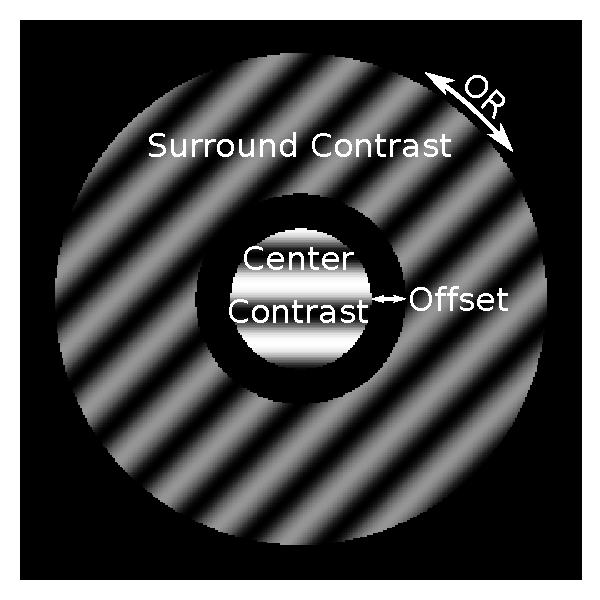
\includegraphics[width=0.5\textwidth]{ORC_Stimulus.pdf}
	\caption{orientation-contrast stimulus measuring modulation by a
      sine grating annulus on the response of a central neuron
      responding to a central sine grating disk of the same frequency.
      Stimulus is varied by center and surround contrast, surround
      orientation and the offset between the central disk and the
      surround annulus.}
	\label{ORC_Stimulus}
\end{figure}

The surround facilitation is quantified as:

\begin{equation}
F = (\frac{R_{cs}}{R_c} - 1) 100
\end{equation}

where $R_{CS}$ is the response of the combined stimulus and $R_C$ the
response to just the center stimulus.

\paragraph{Pop-out}

One of the most well studied effects in the surround-modulation
literature is the pop-out effect, where when a visual stimulus is
embedded within a number of dissimilar features it strongly stands
out. It is thought this effect relies on similar features suppressing
each other leaving the dissimilar unaffected and therefore
``popping-out`` of the background \citep{Kastner1997}. In order to
test this surround-modulation effect we generate visual patterns
container a target bar stimulus surrounded by a circle of flanker
stimuli, which are either co-aligned with the target (iso-condition)
or orthogonal to the target (cross-condition).

The response to the targets and the flankers is then computed as the
mean activity of the non-zero responding units with two annuli one
covering the central 1 degrees and the other covering the remaining
simulated area.

\section{Results}

As previously discussed the surround-modulation effects in the model
are highly dependent on the statistics of the visual input the model
was trained on. Since the standard Gaussian patterns used so far do
not exhibit any long-range correlations the analyses here will use
models trained on natural images, which itself has some drawbacks,
however it allows the model to learn the statistics of the natural
world or of various laboratory environments. The following analyses
all use either the ``natural`` or the ``treeshrew`` dataset shown in
\ref{image_patterns}.

\subsection{orientation-contrast suppression}

Orientation-contrast suppression is one of the most well-studied
paradigms in the surround-modulation literature. One of the most
thorough analyses was performed by \cite{Jones2002}, varying the
relative size and offset of the center stimulus and surround
annulus. In our analysis the contrast suppression will not be
characterized to the same extent. The measurements were performed in
the model trained on the ``natural`` dataset, which does not have as
highly biased statistics as the laboratory datasets.

As a first step the orientation-contrast curve was measured for a
number of randomly chosen neurons under high-contrast conditions and
all non-responding units were rejected. By normalizing the response
and averaging the curves and computing the standard error the average
contrast suppression curve was computed and can be seen compared to
the orientation-contrast suppression curve from a single neuron
measured by \cite{Jones2002} in \ref{ORTC_Jones}. The result shows
that the neurons show strong iso-orientation suppression with a fairly
well defined shape, which does not vary considerably in width.

\begin{figure}
	\centering
        \includegraphics[width=1.0\textwidth]{./results/lespi/ORTC_Jones_Comparison.pdf}
	\caption[Averaged orientation-contrast suppression curve compared
      against \cite{Jones2002} example curve.]{Averaged orientation
      contrast suppression curve compared against \cite{Jones2002}
      example curve. A) Shows the normalized and averaged orientation
      contrast suppression curve from 11 neurons against the average
      orientation tuning curve of the same neurons both with standard
      error bars. B) A sample orientation-contrast suppression curve
      reproduced from \cite{Jones2002}.}
	\label{ORTC_Jones}
\end{figure}

\subsubsection{Contrast Dependence}

In addition to measuring the classical high-contrast suppression
curve, the equivalent measurement was performed for an individual
neuron under both low and high-contrast conditions. The orientation
contrast tuning curves were measured at each settling step of the
model and are shown in \ref{ORTC_ContrastDependence}. As these results
clearly show the neuron exhibits very different effects under the two
conditions. When the local and global contrast is low the response of
the neuron is enhanced while high-contrast stimulation demonstrates
the same suppressive effect that is evident in the averaged
suppression curve in \ref{ORTC_Jones}.

In order to find the cross-over point at which facilitation turns to
suppression the contrast of both the center and surround pattern is
varied and the OCSI is calculated for different durations. The
corresponding plot is shown in \ref{ORTC_ContrastCurve} highlighting
again that suppression weakens as the response is settling but more
important clearly shows the inflection point between excitation and
suppression for this particular neuron lies at about 9\% contrast.

\begin{figure}
	\centering
        \includegraphics[width=0.8\textwidth]{./results/lespi/ORTC_CSContrast.pdf}
	\caption[Contrast dependent switch from facilitation to
      suppression.]{The relationship between contrast and orientation
      contrast suppression. A) Effect of varying center and surround
      contrast on the OCSI, demonstrating a shift from facilitation
      (positive OCSI) to suppression (negative OCSI). B) Effect of
      varying center and surround contrast independently demonstrating
      that both local and surround context influence contextual
      modulation.}
	\label{ORTC_ContrastCurve}
\end{figure}

This analysis also demonstrates how the suppression varies over the
time course of the response, beginning shortly after onset (which
occurs after a duration of about 0.25 and is excluded from analysis)
and peaking at around 0.7 before weakening again. Since there is no
real model of time in this model it is hard to relate this to
experiments but it is clear that long-range effects, resulting from
the integration over a larger area must occur after the
onset. Investigating the precise timecourse of the different cell
classes will make it clearer how the contrast dependence of the
surround modulation emerges from the circuit.

\begin{figure}
	\centering
        \includegraphics[width=1.0\textwidth]{./results/lespi/ORTC_ContrastDependence.pdf}
	\caption[Dependence of orientation-contrast suppression on local
      and global contrast.]{Dependence of orientation-contrast
      suppression on local and global contrast. A, C) Low- and
      high-contrast orientation-contrast suppression patterns. B, D)
      Corresponding orientation-contrast suppression curves showing
      facilitation at low contrast and suppression at high contrast
      respectively.}
	\label{ORTC_ContrastDependence}
\end{figure}

\subsubsection{Spatial dependence}

As the LESPI model has inherited the spatial calibration from the
previous models we can directly relate the extent of surround
suppression in the model to the cortex, allowing us to draw
conclusions about the surround modulation. In doing so we are only
limited by the area that can feasible simulated in the model. We
therefore vary the offset between center pattern and the surrounding
annulus and measure the effect on the OCSI.

\begin{figure}
	\centering
        \includegraphics[width=0.5\textwidth]{./results/lespi/ORTC_Offsets.pdf}
	\caption[Spatial dependence of surround suppression.]{The
      relationship between the distance between the center pattern and
      the surrounding annulus on the OCSI, demonstrating a slow
      falloff in surround suppression strength as the surround
      suppression stimulus is moved further away from the central stimulus.}
	\label{ORTC_OffsetCurve}
\end{figure}

\subsubsection{Timecourse}

In order to get a better understanding of how the different cell
classes and synaptic projections interact to give rise to the
contextual modulation effects seen above the timecourse of the
activity can be visualized. The timecourse of the responses under four
different conditions is shown in \ref{ORTC_Timecourse}. The top-row
shows the response under low-contrast conditions for the
iso-orientation and cross-orientation condition and highlights how the
iso-orientation facilitation emerges. Comparing A and B it is clear to
see how the lateral excitation increases the excitatory response in
the iso-orientation condition but activates more weakly in the
cross-orientation condition. Similarly in the high-contrast case the
Sst population activates much more strongly in the iso-orientation
condition (C) than in the cross-orientation condition.

\begin{figure}
	\centering
        \includegraphics[width=1.0\textwidth]{./results/lespi/ORTC_TimeCourse.pdf}
	\caption[Time-course of neural and synaptic projection responses
      under four conditions, demonstrating how a contrast-dependent
      switch between facilitation and suppression occurs]{Time-course
      of neural and synaptic projection responses under four
      conditions, demonstrating how a contrast-dependent switch
      between facilitation and suppression occurs. A) In low contrast
      iso-orientation condition lateral excitation exceeds the
      activation of the V1 Sst population resulting in
      facilitation. B) In low contrast cross-orientation condition
      very little surround modulation occurs. C) In high-contrast
      iso-orientation condition the Sst population activates strongly
      causing strong suppression. D) Under high-contrast
      cross-orientation condition Sst neurons are only weakly
      recruited resulting in moderate amount of modulation.}
	\label{ORTC_TimeCourse}
\end{figure}

\subsection{Flanker Modulation}

A second often used paradigm to measure surround-modulation effects is
presenting a target stimulus optimized for a particular neuron and
then adding flanker stimuli, which vary in orientation from the
central neuron. These patterns are much more sparse and therefore do
not engage the circuitry in the same way a natural image stimulus or
even sine grating stimulus would. We are particularly interested
whether the surround-suppression effects that were seen above are
sufficient to account for various saliency-based computations that are
thought to originate in the early visual cortex. Specifically whether
iso-orientation suppression can drive a pop-out effect where visual
elements with similar orientations suppress each other, which will
leave any heterogeneous elements unaffected.

The simplest means of testing this effect was to embed a target bar
stimulus in a ring of iso- or cross-oriented flankers and computing
the average activity in the region corresponding to the flanker
against the region corresponding to the target for the target. The
effect of this can be seen in \ref{Flanker_PopOut}, showing the two
stimulus conditions and a plot of the average in the central target
region and in an annulus around it corresponding to the flanker
region. The target activity is elevated above both the flanker
activation in the same stimulus condition but is also elevated more
importantly is also elevated when compared to the iso-orientation
condition where all flankers have the same orientation.

\begin{figure}
	\centering
        \includegraphics[width=1.0\textwidth]{./results/lespi/Flanker_Popout.pdf}
	\caption[Pop-out effect in simple flanker paradigm.]{Demonstration
      of pop-out effect by presenting target with either
      iso-orientated or cross-oriented flankers and averaging the
      response in two annuli corresponding to the target and flanker
      region. Shows the V1Exc sheet responses, colored by the
      orientation preference of the neurons. The averaged responses
      highlight pop-out of the target stimulus from the background in
      the cross-orientation condition but not the iso-orientation
      condition.}
	\label{Flanker_PopOut}
\end{figure}

\section{Discussion}

In this chapter we introduced the LESPI model as an extension of the
models presented in previous chapters and demonstrated how the model
can mediate many of the contextual modulation effects that are known
to occur in the primary visual cortex. Unlike many other 
surround-modulation models this model explains mechanistically how the
long-range patchy excitatory connections emerge in the model and how a
specific class of inhibitory neurons can explain contrast and context
dependent changes in surround modulation.

Specifically using standard experimental paradigms for assessing the
surround modulation in the primary visual cortex we show that the
combination of long-range lateral connectivity targetting both
excitatory and inhibitory neurons can provide a good match to
electrophysiological and psychophysical results. It also allows
inspecting the responses of every single neuron providing a much more
comprehensive view of how neural responses are modulated.

\subsection{Feature dependent modulation}

There are a wide range of models that have been used to explain
feature specific surround modulation effects in the visual
cortex. These models usually start by modeling a number of feature
detectors, which are connected according to their similarity in the
feature space \citep{Li2002, Schwabe2006}. When modeling V1 this
usually means connecting neurons with similar orientation preference
to replicate the effect of the long-range patchy connectivity, which
is known to link iso-orientation columns. However, while such models
are useful to study specific phenomena they provide an unsatisfying
and narrow explanation of cortical function, which does not generalize
across different brain regions and sensory modalities.

Developmental models such as the model presented here explain the
emergence of surround modulation effects as a consequence of the way
the circuit self-organizes and learns the statistics of the natural
world. In other words, unlike other models none of the surround
modulation effects are hard-coded, instead they emerge naturally due
to simple mechanisms including Hebbian learning, divisive gain control
and homeostasis and the interactions between different cell
classes. The existence of iso-orientation facilitation and suppression
is therefore the result of the model extracting co-occurrences in the
training patterns. Indeed by comparing models trained on simple
independent Gaussian patterns, with the same model trained on natural
or laboratory images, it is clear that the long-range modulatory
effects only emerge when the training patterns contain consistent
long-range correlations.

This adds to the growing amount of literature suggesting that the
cortex uses the statistical dependencies between sensory features to
optimize neural coding \citep{Vinje2000, Simoncelli2001} and improve
performance in specific tasks \citep{Geisler2001}. In the LESPI model
the long-range connections learn a statistical distribution of the
inputs and can modulate the response to give rise to both facilitatory
effects and suppressive effects. This effect is mediated through a
divisive normalization mechanism, strongly resembling other models,
which use higher-order correlations to optimize neural coding by
reducing redundancy \citep{Spratling2011, Coen2015}. This work
suggests that the patchy lateral connections in primary visual cortex
could be the first stage for this computation without requiring
specific feedback from higher level areas. In how far they contribute
to decorrelating activity and influence development requires further
characterization however.

At the same time the spatial scales over which the lateral connections
can effectively act are very limited dropping off almost completely
after about $1^\circ$ in visual angle in the model. This suggests that
the lateral connections could mediate effects at the borders of
different textures and perhaps at higher eccentricities where they
cover a much larger visual area.

Some previous theoretical models have provided models of surround
modulation that approach the problem at a more computational level. In
particular there is growing amounts of evidence that the sensory
cortices make use of the statistical relationships in their inputs to
optimize the representation

\subsection{Contrast-dependent changes in suppression}

The contrast-dependence of surround modulation effects has been of
great interest for a long time and a number of models have been
proposed to explain it. Specifically some form of assymetry between
excitatory and inhibitory neurons is required as \cite{Somers1998}
suggested. Their original proposal relied on an assymmetry in
thresholds between excitatory and inhibitory, which is only supported
by limited evidence. However they also suggested that
excitatory-inhibitory connections which increase in efficacy under
strong stimulation in contrast to excitatory-excitatory connections,
which seemingly integrate sublinearly with increasing contrast
\citep{Abbott1997, Tsodyks1997}, could account for this assymmetry.

Since then a large number of studies have focused on different classes
of inhibitory neurons and the Sst suppressing interneurons fit
precisely this description. Not only does the model demonstrate the
contrast dependent switch from facilitation to suppression that has
been so widely described \citep{Hirsch1991,Weliky1995, Toth1996} as
can be seen in \ref{ORTC_ContrastCurve} and \ref{ORTC_CSCurve}, but
we can directly observe how the assymetry in the efficacy of
excitatory-excitatory and excitatory-inhibitory connections targetting
the excitatory and Sst populations respectively drives both phenomena
in \ref{ORTC_ContrastDependence}.

In the model the long-range projections integrate over both space and
time due to their large spatial scale and hysteresis, effectively
computing based on the local stimulus drive and the contextual
activations whether to suppress or enhance the neural response. While
the contrast interactions have been characterized well and correspond
well with experimental results, further analysis should focus on how
modulating the strength affects the sparsity of responses thereby
influences the developmental processes in the model.

\subsection{Spatial dependence}

One of the major features of this model over previous models is the
calibration of spatial profiles of connectivity. This of great
importance to understand the contributions to surround modulation
effects in the cortex. A lot of work has focused on teasing apart the
contributions of lateral connectivity and feedback connections to
surround suppression \citep{Angelucci2002, Bair2003, Schwabe2006}. As
many other studies suggest the LESPI model demonstrates that while the
lateral connections can mediate significant surround modulation
effects, there relatively small spatial scales, covering up 6-7 mm in
total diameter, translating to a visuotopic extent of about
$2.5^\circ$, is not sufficient to account for true long-range surround
suppression which can subtend more than $7^\circ$ in visual angle
\citep{Bair2003, Levitt2002}.

Therefore the lateral connections modeled here cannot account for the
full extent of surround modulation. At the same time it is likely that
they do provide some integration to take into the account the local
context of the receptive field, perhaps aiding in computing the
continuation of a contour or increasing the saliency of borders
between different textures. Further experimental work should focus on
considering the relationship between the neurons receptive field size
and the extent of its lateral connections as that would provide a
clearer indication whether the lateral connections are involved purely
in local processing in the classical RF or also mediate non-classical
receptive field effects. Indeed since this relationship varies
considerably between species, that the role of lateral connections
could also be to a large part species dependent. In species with a
smaller cortex these connections can span a considerable fraction of
the visual field and could therefore mediate even long range surround
modulation effects, while in species with larger brains such as
macaques their role would be limited to near-surround suppression.

\subsection{Temporal scales}

In the current model the temporal properties of the neurons is only
modeled on a very coarse level. Nonetheless the classical shape of
PSTHs emerges naturally from the model. Combining this model with
temporally calibrated models as developed in \citep{StevensPhD2016}
would shed more light on the propagation speeds of the lateral
connections, however based on a rough calculation the long-range
projections propagate at a speed of up to 0.2 m/s, in the model which
is well within the physiological range of 0.1-0.3 m/s. This means the
surround modulation arriving from lateral connections act fast enough
to have an effect, however any longer range effects would have to be
mediated by longer range connections.

The spatial scales of surround modulation are of great interest as
well as there is a lot of discussion centered around the question of
where these effects originate. As the model that we are using has been
spatially calibrated we can make concrete predictions about the
spatial extents to which lateral connections in layer 2/3 could
mediate surround suppression.

\subsection{Simple and Complex cells}

One major limitation of the current model is the lack of complex
cells, which causes disruptions to the map organization when trained
on natural images. This also means that neurons respond optimally at
one particular phase, so all surround modulations are dependent on the
phase of the stimuli. In future the model could be extended to
incorporate layer specific circuits allowing the emergence of complex
cells and improving the organization of the orientation map as has
been demonstrated previously \citep{Antolik2010}. This is of
particular interest because it is unclear to what extent lateral
connections will capture the relative phase between different edges if
they are primarily connecting complex cells in layer 2/3, which could
haave strong implications for their ability to represent specific
spatial arrangements and mediate contour integration effects. This is
a very important question and more experimental work should focus on
the differences in lateral connections in simple and complex cells.

\subsection{Development}

In this chapter we mainly examined the role of lateral connectivity in
surround modulation effects. In the current model the lateral
connections are simulated as initially diffuse connections, which
organize a patchy architecture connecting iso-orientation regions
after development and finally they are thresholded as to reflect the
highly sparse organization that is observed in tracing studies. This
is likely not a good approximation of their actual development, as
they do not emerge until after development. It also partially disrupts
the organization of the model as the initially diffuse and isotropic
connections introduce destructive long range correlation to the model
\citep{Miikkulainen2005}.

As part of this thesis a sparse matrix implementation of the core
algorithms was implemented, along with a variety of sprouting and
retraction algorithms. In future a more realistic approach to model to
match the timecourse of lateral connectivity development, which begins
after the emergence of an orientation map \citep{Ruthazer1996}, should
be developed based on these early explorations. Initial results
suggested that most sprouting and retraction approaches could produce
equivalent orientation maps and often resulted in more selective and
stable tuning properties.

Additionally it is interesting to consider how reducing the
correlations between distant neurons using surround suppression
affects learning in the model. While decorrelating the activity of
feedforward components will help in maintaining an unbiased
distribution and therefore good coverage of features, it also reduces
the precise correlations it is trying to learn. In other words if the
long-range suppression reduces correlations in the input it is
eliminating the exact thing it is trying to capture. Indeed through
initial investigation in the model we were able to show that
increasing the strength of lateral excitatory connections targetting
the Sst population reduces the strength of both iso-orientation biases
and isotropy biases. This suggests that the lateral connections might
learn differently from afferent connections, i.e. that afferent
connections should learn on the final settled response, while the
lateral connections should strengthen depending on the coherence of
the signals arriving from afferent and lateral connections. Indeed
this provides an interesting connection to predictive coding models
\citep{Rao1999}, where the sign of the lateral modulation represents
the sign of the error. If the lateral excitatory-inhibitory
connections were to strengthen in the facilitatory regime and
excitatory-excitatory connections were enhanced in the suppressive
regime. In other words the difference between lateral excitation and
lateral inhibition encodes an implicit error in the prediction of the
model, which could be used to adjust the lateral connectivity to more
accurately reflect the statistics of the input.

\subsection{Effects of natural image statistics on the model}

In this chapter we switched from simple Gaussian patterns for training
the model to samples from natural images, to allow the model to learn
co-occurrence statistics in the lateral connections, which give rise
to the surround modulation effects observed here. However the
statistics of various natural image datasets can differ considerably
and relating the statistics of the sensory environment an animal is
reared in and the surround modulation effects would be a huge step
forward in understanding how the cortex learns higher-order
correlations in the natural world.

Before such an analysis can be performed we have to robustly quantify
the statistics of the natural image patterns and what the lateral
connections have actually learned before relating these observations
back to specific surround modulation results in the psychophysics and
electrophysiology literature. In the next chapter we will present
various analyses to do precisely that, which will let us make concrete
predictions of how the visual rearing environment affects the
processing of simple and complex stimuli.
